Denne sektion diskuterer det proof of concept, der blev lavet til aktivitetsdelen af projektet, samt diskuterer hvordan data aggregeres og hvilket videre arbejde der kan være nyttigt. 
Idéen ved at lave et proof of concept til fysisk aktivitet er at det er en lavt hængende frugt, som nemt kan implementeres, hvorefter vi forventer den kan arbejdes videre på, på et senere tidspunkt. 
Det er dog vigtigt at selvom vi ikke bruger meget tid på denne del, understreger vi at ændringer i fysisk aktivitet er meget vigtigt, når det kommer til affektive lidelser. 

Metoden der bruges til at måle fysisk aktivitet blev valgt til at være skridttælleren, da den tilnærmer sig fysisk aktivitet, idet at hvis man bevæger sig meget vil ens skridttæller afspejle dette.
Da skridttælleren regnes for en lavthængende frugt ses der blot på denne løsning, men med videre arbejde kan andre løsninger udforskes.

Et eksempel på dette kunne være at dobbelt integrere accelerationsmålinger til at få et andet mål for fysisk aktivitet.
Ved at dobbelt integrere acceleration fås et mål for strækning, og på den måde kan det regnes for fysisk aktivitet.
Fordelen ved at bruge en sådan løsning fremfor GPS for eksempel, ville være at det højst sandsynligt er billigere i strøm, samt at man ikke behøver gå en tur for at det registreres. Aktiviteter der foretages på samme spot vil dermed også kunne registreres.
Det er modsat skridttælleren ikke begrænset til en bestemt type bevægelse, og ses derfor som en klar fordel.
Imidlertid er skridttælleren allerede tilråd i Android, og er derfor brugt som en første tilgang.
Tilgangen med at dobbelt integrere regnes dog ikke for værende meget sværere at implementere, og bør derfor arbejdes videre på med mere udviklingstid.

Eftersom skridttælleren bruges, er det eneste, der skal gøres for at indsamle data, at lave et sensor modul.
Sensor modulet skal derved kun bruge den indbyggede skridttæller i Android smartphones.
Derefter skal et analysemodul laves, der kan lave en aggregering af alle ens skridt for en given dato.

\subsection{Aggregering}
For at informationen samlet af skridttælleren kan være brugbar, skal den samles på en eller anden måde.
Her vælges det at samle data for hver eneste dag, altså at alle målinger fra starten af en dag til slutningen af den samme dag bliver summeret til en værdi.

\subsection{Visualisering}\label{sec:aktivitetVis}
Der er brug for at vise brugeren hvor mange skridt de har gået i løbet af en dag.
Denne visualisering skal kunne bruges af brugerne til at se hvor mange skridt de har gået på en bestemt dato, men også hvordan deres antal af skridt ændrer sig i løbet af en længere periode.

For at give et sådant overblik, er der blevet lavet et søjlediagram, hvor hver søjle viser hvor mange skridt man har gået på en bestemt dato, et eksempel kan ses i \cref{fig:skridttaeller}.
Dette kan dog nemt komme til at se uoverskueligt ud hvis man har data for et helt år, hvilket er grunden til at zoom er blevet introduceret.
Denne funktionalitet gør at det er nemt for brugerne at få et overblik over hvordan deres antal af skridt ændres i løbet af en kort periode, men også hvordan det ændres over en længere periode.
Dette gør det nemmere for brugerne at danne et overblik over hvordan deres adfærd ændres.

\begin{figure}[h]
	\centering
	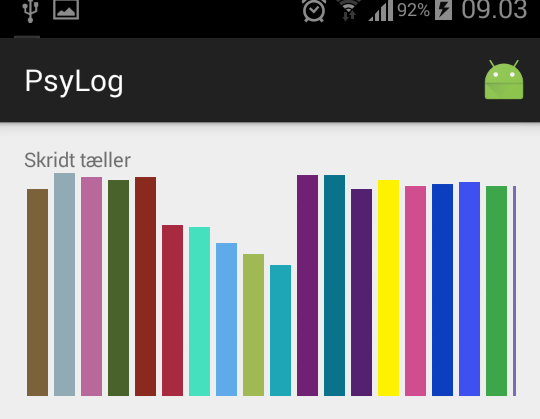
\includegraphics[scale=0.6]{visningbarchart}
	\caption{Visualisering af skridttæller.}
	\label{fig:skridttaeller}
\end{figure}